\documentclass[11pt,letterpaper]{article}
\usepackage[lmargin=1in,rmargin=1in,tmargin=1in,bmargin=1in]{geometry}
\usepackage{../style/homework}
\usepackage{../style/commands}
\setbool{quotetype}{false} % True: Side; False: Under
\setbool{hideans}{true} % Student: True; Instructor: False

% -------------------
% Content
% -------------------
\begin{document}

\homework{10: Due 04/14}{There is geometry in the humming of the strings; there is music in the spacing of the spheres.}{Pythagoras}

% Problem 1
\problem{10} Find the angles marked $x$, $y$, and $z$ in the triangle given below. 
	\[
	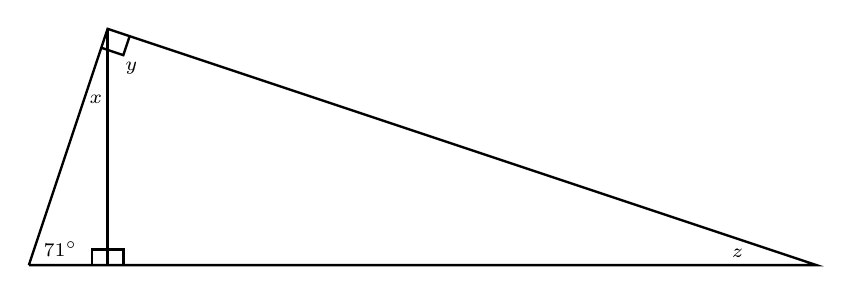
\begin{tikzpicture}
	\draw[line width=0.03cm] (0,0) -- (1,3) -- (10,0) -- (0,0);
	\draw[line width=0.03cm] (1,3) -- (1,0);
	\draw[line width=0.03cm] (0.8,0) -- (0.8,0.2) -- (1.2,0.2) -- (1.2,0);
	\draw[line width=0.03cm] (0.92,2.76) -- (1.2,2.666) -- (1.2802,2.9066);
	\node at (0.4,0.2) {\scriptsize$71^\circ$};
	\node at (0.85,2.1) {\scriptsize$x$};
	\node at (1.3,2.5) {\scriptsize$y$};
	\node at (9,0.15) {\scriptsize$z$};
	\end{tikzpicture}
	\]



\newpage



% Problem 2
\problem{10} Find $x$ in the following figure:
	\[
	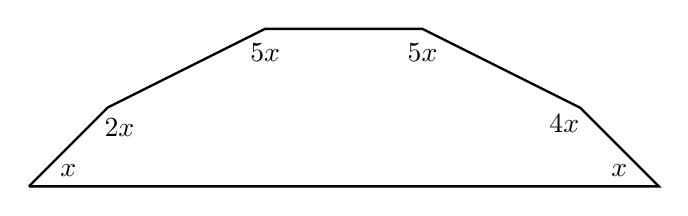
\begin{tikzpicture}
	\draw[line width=0.03cm] (0,0) -- (1,1) -- (3,2) -- (5,2) -- (7,1) -- (8,0) -- (0,0);
	\node at (0.5,0.2) {$x$};
	\node at (1.15,0.75) {$2x$};
	\node at (3,1.7) {$5x$};
	\node at (5,1.7) {$5x$};
	\node at (6.8,0.8) {$4x$};
	\node at (7.5,0.2) {$x$};
	\end{tikzpicture}
	\]



\newpage



% Problem 3
\problem{10} A simple closed curve is plotted below. Determine whether the red point is located on the interior or the exterior of the curve. Be sure to justify your answer.
	\begin{figure}[!ht]
	\centering
	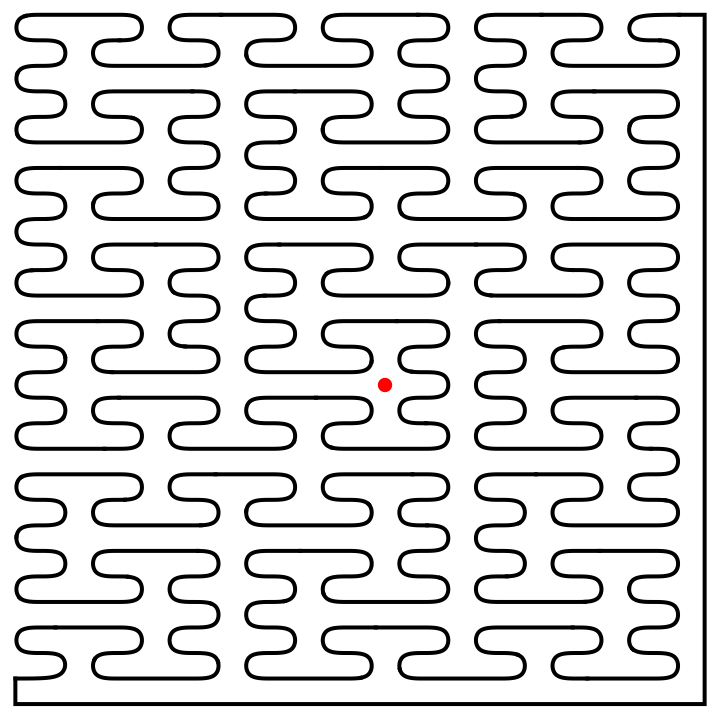
\includegraphics[width=0.5\textwidth]{peanocurve.png}
	\end{figure}


\end{document}